\documentclass{article}

% Language setting
% Replace `english' with e.g. `spanish' to change the document language
\usepackage[spanish]{babel}

% Set page size and margins
% Replace `letterpaper' with `a4paper' for UK/EU standard size
\usepackage[letterpaper,top=2cm,bottom=2cm,left=3cm,right=3cm,marginparwidth=1.75cm]{geometry}

% Useful packages
\usepackage{amsmath}
\usepackage{graphicx}
\usepackage[colorlinks=true, allcolors=blue]{hyperref}

\title{Simulación de Eventos discretos}
\author{Jossué Arteche Muñoz \\ C311}

\begin{document}
\maketitle

\section{Introducción}

Este proyecto consiste en la implementación y análisis del procesamiento de paquetes de un centro de clasificación postal, donde los paquetes que llegan desde distintas oficinas o buzones deben pasar por un proceso de clasificación en dos etapas antes de ser despachados a su destino: registro del paquete y clasificación automática. Para ello se modeló el problema como un sistema con dos servidores en serie, donde los paquetes arriban al sistema según un proceso de Poisson no homogéneo.

\subsection{Objetivos y metas}
El objetivo fundamental del proyecto es simular de manera lo más precisa posible el comportamiento del sistema para estudiar su rendimiento bajo determinadas suposiciones iniciales. Entre las metas propuestas se encuentran:

\begin{itemize}
\item Implementar una simulación basada en eventos discretos del sistema de dos servidores en serie.
\item Incorporar una política de llegadas no homogéneas mediante el método de aceptación-rechazo
\item Medir variables clave como el tiempo de estancia de un paquete en el sistema, el tiempo total, etc.
\item Realizar pruebas de hipótesis con intervalos de confianza, auxiliándose la técnica del bootstraping
\item Evaluar el desempeño del sistema a partir de la visualización y análisis de los resultados obtenidos
\end{itemize}

\subsection{Variables de interés y asunciones iniciales}
Entre las variables de interés que se analizarán, se incluyen:

\begin{itemize}
    \item Tiempo de llegada al sistema.
    \item Tiempo total en el sistema por cliente.
\end{itemize}

El modelo del problema depende de las siguientes variables:

\begin{itemize}
    \item $\lambda(t)$: función de intensidad de llegadas, dependiente del tiempo $t$ expresado en minutos.
    \item $\lambda_{\text{max}}$: cota superior de $\lambda(t)$, usada para la generación de llegadas por el método de aceptación rechazo.
    \item $T$: tiempo de cierre del sistema.
    \item $G_1$ y $G_2$: variables generadoras del tiempo de respuesta de los servidores.
\end{itemize}

\section{Detalles de la implementación}

El modelo fue implementado en el lenguaje Python, usando el intérprete Python 3. Se utilizaron como dependencias fundamentales las librerías numpy y matplotlib. La mayor parte del modelo simulado se encuentra en la clase TandemSystem, la cual toma como parámetros las dependencias del modelo. También se creó un archivo de funciones útiles para realizar algunos análisis y generar gráficas estadísticas. En el archivo main.py se encuentra el punto de entrada de la simulación, así como el código generador de los gráficos de este informe.

\section{Resultados y experimentos}

Para construir un modelo realista y manejable del sistema de procesamiento postal en un centro de clasificación, se han adoptado las siguientes suposiciones: 

\begin{itemize}
    \item Se ha tomado como función de intensidad la $\lambda(t) = 2e^{-t/240}$, que modela un flujo más intenso al inicio de la jornada, disminuyendo progresivamente con el tiempo. Esta decisión refleja un centro de correos en el que el flujo de trabajo es mayor en las horas de la mañana. Tomada esta función resulta conveniente tomar $\lambda_{\text{max}} = 2$ como cota superior de la función de intensidad.
    \item Se ha tomado $T = 480$ para simular una jornada de 8 horas.
    \item Se asume que los tiempos de atención siguen las distribuciones $G_1 \sim \mathcal{N}(\mu = 0.5, \sigma^2 = 0.25)$ y $S_1 \sim \mathcal{N}(\mu = 0.6, \sigma^2 = 0.25)$. Se tomaron para simular un sistema rápido y automatizado
\end{itemize}

Al ejecutar la simulación de un centro de procesamiento postal durante una jornada laboral de 480 minutos, se registraron los tiempos de estancia de cada paquete en el sistema. El total de consumidores procesados fue significativo, permitiendo extraer conclusiones estadísticas relevantes. Obtenemos el histograma de la figura \ref{Figura1}, el cual nos muestra la media y la mediana de los tiempos de estancia de paquetes en el sistema.

\begin{figure}
    \centering
    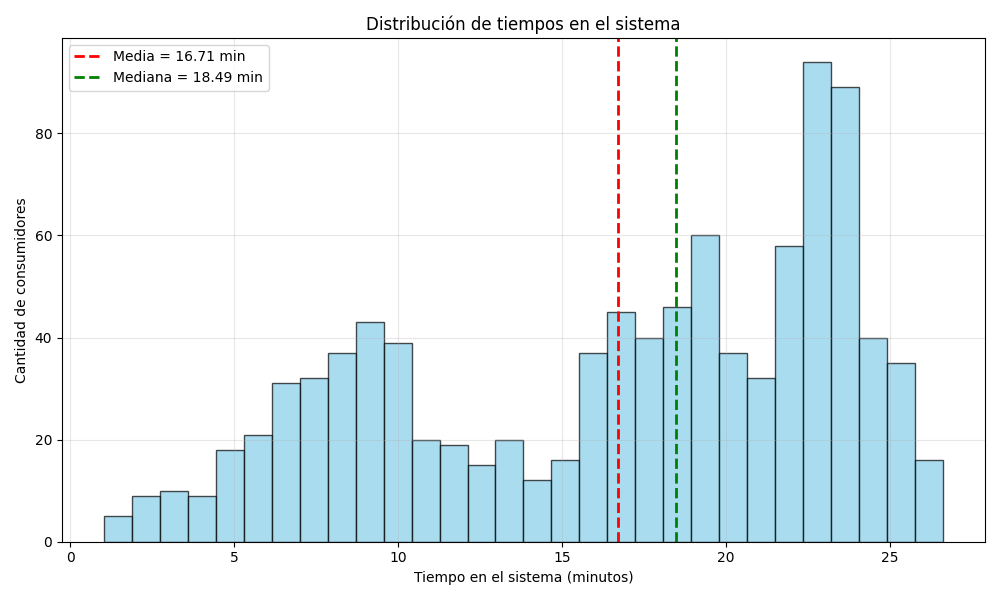
\includegraphics[width=1\linewidth]{tiempos_en_sistema.png}
    \caption{Tiempos de estancia de paquetes en el sistema}
    \label{Figura1}
\end{figure}

Se observaron las siguientes medidas de tendencia central:

\begin{itemize}
    \item Media del tiempo en el sistema: 16.71 minutos
    \item Mediana del tiempo en el sistema: 18.49 minutos
\end{itemize}

Se observa que los valores medios y la dispersión de los tiempos indican que el sistema, en su configuración actual, logra mantener un tiempo medio en el sistema inferior a los 18 minutos, lo cual podría considerarse eficiente para un centro de clasificación postal.

\subsection{Pruebas de hipótesis}
Se plantearon dos hipótesis estadísticas basadas en los datos obtenidos de la simulación. Ambas están formuladas para comprobar si los consumidores permanecen en el sistema más de 17 minutos en promedio y en casos típicos (mediana).

Para validar estas hipótesis, se empleó la técnica de bootstrap, generando 1000 remuestreos con reemplazo de los tiempos en el sistema registrados durante la simulación.

\subsubsection{Hipótesis 1 – Tiempo promedio en el sistema}

\begin{itemize}
    \item $H_0$ (hipótesis nula): El tiempo promedio en el sistema es menor o igual a 17 minutos.
    \item $H_1$ (hipótesis alternativa): El tiempo promedio en el sistema es mayor a 17 minutos.
\end{itemize}

Los resultados del bootstraping para esta hipótesis se muestran en la figura \ref{mean-bootstrap}:

\begin{itemize}
    \item $ \text{IC}_{95\%} = [16.26,\ 17.11] $
    \item El valor 17 se encuentra dentro del intervalo de confianza, lo que indica que no hay suficiente evidencia para rechazar la hipótesis nula con un 95\% de confianza.
\end{itemize}


Conclusión: No se puede afirmar que el tiempo promedio en el sistema sea mayor a 17 minutos.

\begin{figure}
    \centering
    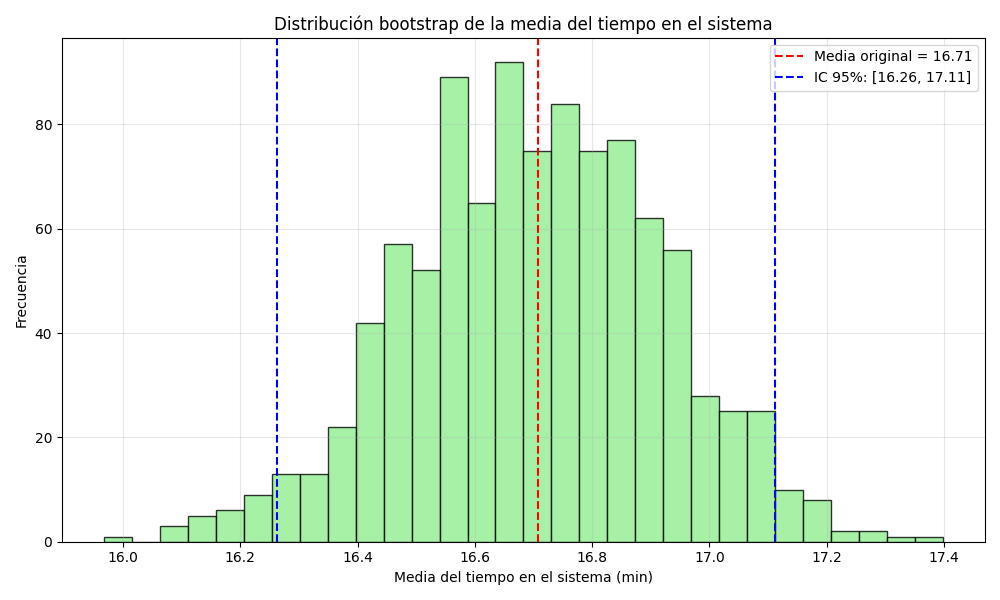
\includegraphics[width=1\linewidth]{bootstrap_media_tiempo.png}
    \caption{Resultados del bootstraping sobre la mediana}
    \label{mean-bootstrap}
\end{figure}

\subsubsection{Hipótesis 2 – Mediana del tiempo en el sistema}

\begin{itemize}
    \item $H_0$ (hipótesis nula): La mediana del tiempo en el sistema es menor o igual a 17 minutos.
    \item $H_1$ (hipótesis alternativa): La mediana del tiempo en el sistema es mayor a 17 minutos.
\end{itemize}

Los resultados del bootstraping para esta hipótesis se muestran en la figura \ref{median-bootstrap}:

\begin{itemize}
    \item $ \text{IC}_{95\%} = [17.76,\ 18.95] $
    \item El valor 17 está fuera del intervalo de confianza, por lo que se puede afirmar con un 95\% de confianza que la mediana supera ese umbral.
\end{itemize}

\begin{figure}
    \centering
    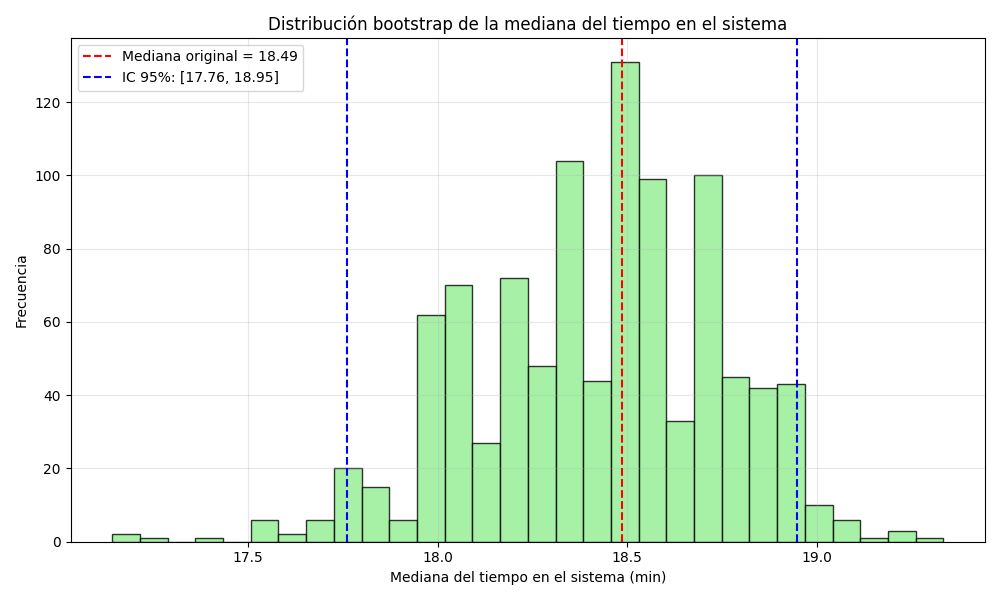
\includegraphics[width=1\linewidth]{bootstrap_mediana_tiempo.png}
    \caption{Resultados del bootstrapping para la mediana}
    \label{median-bootstrap}
\end{figure}

Esta combinación de resultados revela que, aunque el tiempo promedio podría no superar los 17 minutos, la mayoría de los consumidores sí lo hace (mediana $> 17$).

\section{Conclusiones}

Este proyecto evidencia el potencial de la simulación de eventos discretos como herramienta para estudiar el comportamiento de sistemas de servidores en serie, como los centros de clasificación postal. Usando un modelo simplificado, fue posible explorar el impacto de distintas variables de interés, y analizar el desempeño del sistema mediante técnicas estadísticas en un entorno controlado y reproducible.

\end{document}